% IF1014, Relatório final (entrega 10/06/2026, máx. 25 páginas, sem apêndices).
% Compilação: pdflatex relatorio.tex (duas passadas para refs/citações)
\documentclass[12pt,a4paper]{article}
\usepackage[utf8]{inputenc}
\usepackage[T1]{fontenc}
\usepackage[brazil]{babel}
\usepackage[margin=2.4cm]{geometry}
\usepackage{graphicx}
\usepackage{booktabs}
\usepackage{array}
\usepackage{xcolor}
\usepackage{hyperref}
\usepackage{caption}
\usepackage{subcaption}
\usepackage{listings}
\usepackage{amsmath}

\hypersetup{colorlinks=true, urlcolor=blue, linkcolor=black, citecolor=black}

\title{Previsão de readmissão hospitalar em pacientes diabéticos\\\large IF1014, Mineração de Dados Aplicada (CRISP-DM)}
\author{João Pontes \and Marcos Antonio \and Theo Barza \\ UFPE, 2026.1}
\date{10 de junho de 2026}

\begin{document}
\maketitle

\begin{abstract}
Aplicamos o ciclo CRISP-DM completo ao dataset Diabetes 130-US Hospitals (UCI 296) para classificar a janela de readmissão hospitalar de pacientes diabéticos em \texttt{<30}, \texttt{>30} e \texttt{NO}. O conjunto foi dividido por amostragem estratificada uma única vez ($n_{\text{treino}}=81{,}412$, $n_{\text{teste}}=20{,}354$), e o teste foi mantido isolado por uma guarda de token até a avaliação final. Treinamos os 10 algoritmos obrigatórios sob 5-fold estratificado pareado e busca de hiperparâmetros, otimizando F1-macro. Comparamos pareadamente o pré-processamento baseline contra quatro variantes (SMOTE, undersampling, RobustScaler, TargetEncoder). O modelo final \emph{Random Forest} (com \texttt{RobustScaler} e \texttt{class\_weight="balanced"}) alcançou F1-macro de \emph{0{,}455} no teste, com bom desempenho na classe majoritária \texttt{NO} (F1=0{,}672) mas recall de apenas 0{,}196 na classe minoritária \texttt{<30}, justamente a de maior custo clínico. Discutimos riscos de viés, monitoramento e gatilhos de retreinamento para deployment.
\end{abstract}

\tableofcontents
\newpage

\section{Business Understanding}
\subsection{Briefing do cliente fictício}

O cliente \emph{SI5 Health} atua no setor de \emph{cuidado hospitalar pós-alta} e precisa de um modelo capaz de \emph{prever a janela de readmissão de pacientes diabéticos na hora da alta}, em que a saída pertença a uma das classes \texttt{<30}, \texttt{>30} ou \texttt{NO}. O sucesso será medido por \emph{F1-macro} sobre o conjunto de teste, com restrição de \emph{tempo de inferência $<200$ ms por paciente, fila de acompanhamento limitada à capacidade operacional do time pós-alta, e custo assimétrico de erro (falso negativo na classe} \texttt{<30} \emph{é o mais grave: leva a readmissão sem suporte)}. As implicações éticas relevantes são \emph{viés histórico em variáveis demográficas (race, age, gender), privacidade de dados clínicos (pseudonimização e retenção mínima), e o uso do escore como apoio, não substituto, à decisão clínica}.

\subsection{Critérios de sucesso e restrições operacionais}
\begin{itemize}
  \item Métrica principal: F1-macro sobre o teste.
  \item Métricas secundárias: balanced accuracy, ROC-AUC e PR-AUC macro multiclasse, métricas por classe.
  \item Métrica operacional crítica: recall(\texttt{<30}).
  \item Capacidade da fila pós-alta: hipótese de $\approx$30 pacientes/dia, calibração de limiar acontece nesse teto.
\end{itemize}

\section{Data Understanding e EDA}
\subsection{Dataset}
Strack et al.\ (2014) consolidaram 101.766 encontros entre 1999 e 2008 em 130 hospitais americanos. Cada linha é uma internação de paciente diabético, com 50 atributos clínicos, demográficos e operacionais. O alvo \texttt{readmitted} é trinário.

\subsection{Distribuição da classe alvo}
A figura~\ref{fig:eda_class} resume a distribuição no treino após o split. A classe \texttt{<30} representa 11{,}2\%, minoritária, motivando F1-macro como métrica.
\begin{figure}[h]
  \centering
  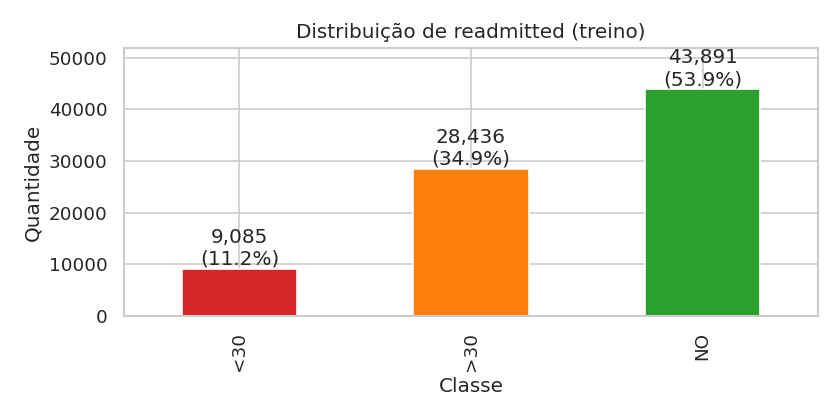
\includegraphics[width=0.62\linewidth]{reports/figures/eda_class_balance.png}
  \caption{Distribuição da classe alvo no conjunto de treino (81.412 pacientes).}
  \label{fig:eda_class}
\end{figure}

\subsection{Missingness e tratamento}
A figura~\ref{fig:eda_miss} elenca colunas com valores ausentes (codificados como \texttt{?} no arquivo bruto). \texttt{weight} (97\%), \texttt{payer\_code} ($\sim$40\%) e \texttt{medical\_specialty} ($\sim$49\%) foram tratadas distintamente: \texttt{weight} foi removida; as demais entraram via imputação \texttt{most\_frequent} no pipeline. As variáveis \texttt{examide} e \texttt{citoglipton} têm um único valor e foram removidas.
\begin{figure}[h]
  \centering
  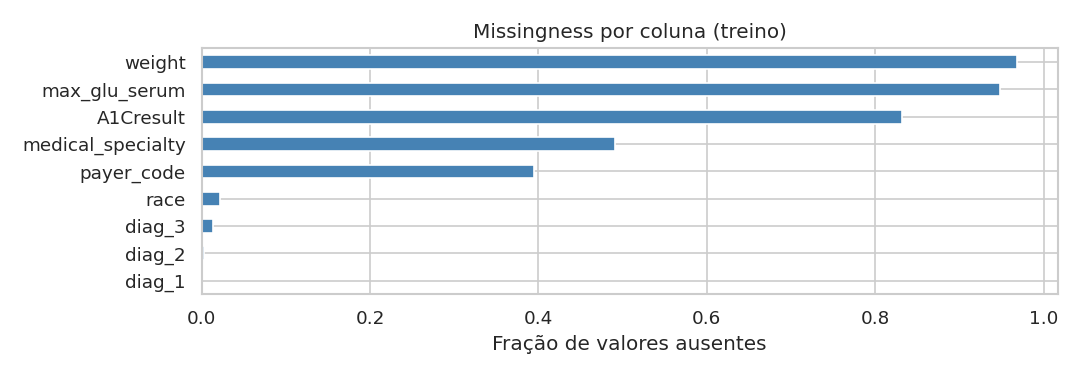
\includegraphics[width=0.7\linewidth]{reports/figures/eda_missingness.png}
  \caption{Fração de valores ausentes por coluna no treino.}
  \label{fig:eda_miss}
\end{figure}

\subsection{Distribuições numéricas por classe}
A figura~\ref{fig:eda_num} mostra que \texttt{number\_inpatient}, \texttt{num\_medications}, \texttt{time\_in\_hospital} e \texttt{number\_diagnoses} diferenciam pacientes \texttt{<30}. As caudas longas em variáveis de contagem motivaram a variante \texttt{RobustScaler}.
\begin{figure}[h]
  \centering
  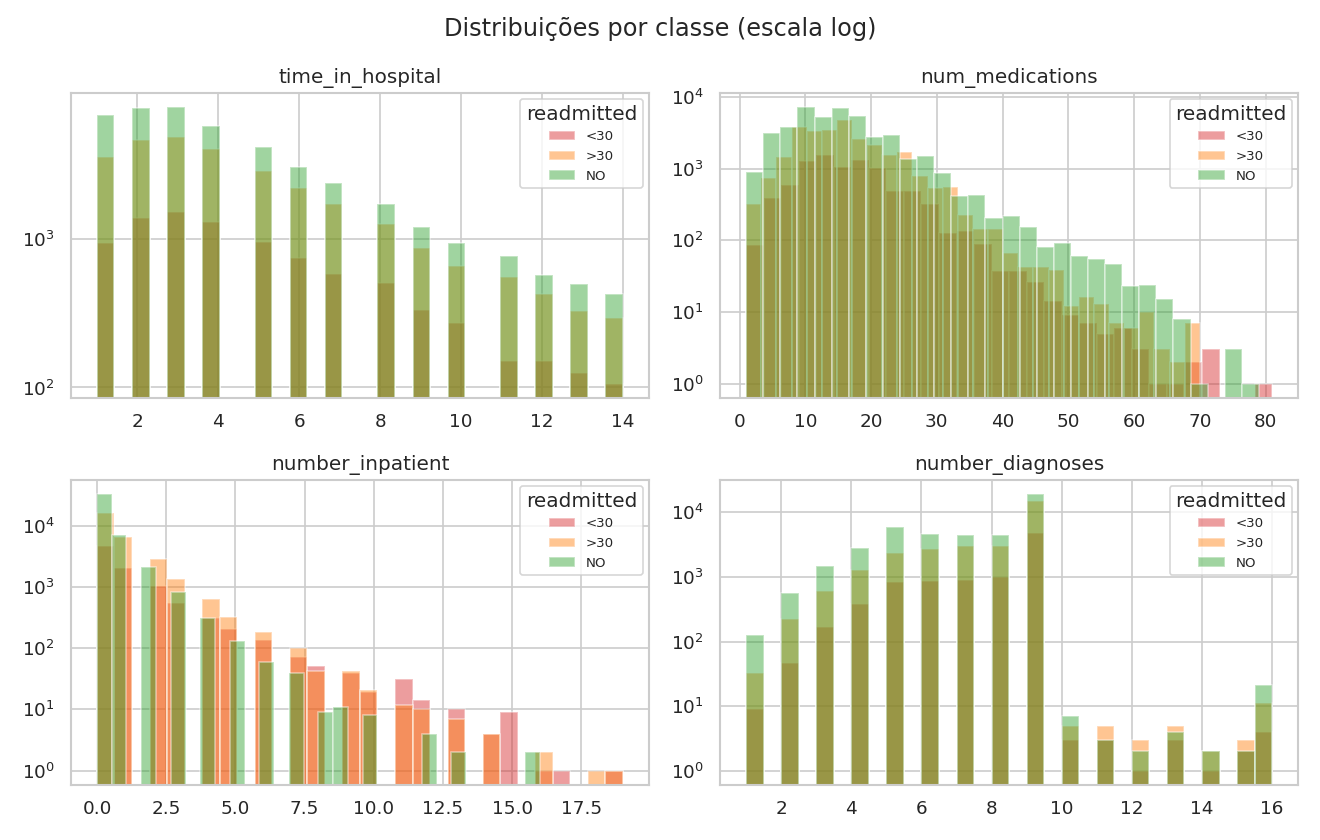
\includegraphics[width=0.85\linewidth]{reports/figures/eda_numeric_by_class.png}
  \caption{Distribuições de variáveis numéricas chave por classe (escala log).}
  \label{fig:eda_num}
\end{figure}

\section{Data Preparation}
\subsection{Integridade do split treino/teste}
O split é materializado em \texttt{data/interim/} com \texttt{random\_state=42}, \texttt{test\_size=0.2} e estratificação. A função \texttt{load\_test} em \texttt{src/data\_loader.py} levanta \texttt{PermissionError} sem o token literal \texttt{I\_AM\_IN\_FINAL\_EVALUATION}. Esse token aparece apenas na Seção 9 do \texttt{main.ipynb}.

\subsection{Pipeline baseline}
\begin{itemize}
  \item \texttt{RawCleaner}: drop estrutural, \texttt{?} $\rightarrow$ NaN, agrupamento ICD-9 (9 categorias clínicas + Other), conversão de IDs operacionais para string.
  \item Numéricas: \texttt{SimpleImputer(median)} $\rightarrow$ \texttt{StandardScaler}.
  \item Categóricas: \texttt{SimpleImputer(most\_frequent)} $\rightarrow$ \texttt{OneHotEncoder(handle\_unknown="ignore")}.
\end{itemize}

\subsection{Variantes}
\paragraph{SMOTE.} \texttt{imblearn.pipeline.Pipeline} com SMOTE aplicado por fold, sintetizando minoria \texttt{<30} via $k=5$ vizinhos.
\paragraph{Undersampling.} \texttt{RandomUnderSampler} dentro do \texttt{imblearn.pipeline.Pipeline}, subamostrando as classes majoritárias por fold para equilibrar o treino. Foi a variante de maior ganho para modelos sem balanceamento embutido (ver a comparação pareada na Seção~5).
\paragraph{RobustScaler.} Substitui StandardScaler nas numéricas. Motivado pela cauda longa em variáveis de contagem.
\paragraph{TargetEncoder.} Codifica \texttt{payer\_code}, \texttt{medical\_specialty}, \texttt{admission\_*\_id} via \texttt{TargetEncoder(target\_type="multiclass")} do scikit-learn (CV interno anti-leakage). Mantém OHE no resto.

\section{Modeling}
\subsection{Os 10 algoritmos}
\begin{table}[h]\centering
\begin{tabular}{lll}
\toprule
\textbf{Família} & \textbf{Algoritmo} & \textbf{Implementação} \\
\midrule
Lazy            & K-NN            & \texttt{KNeighborsClassifier} \\
Protótipos      & LVQ             & \texttt{sklvq.GLVQ} (subclasse \texttt{PatchedGLVQ}) \\
Árvore          & Decision Tree   & \texttt{DecisionTreeClassifier} \\
Margem          & SVM             & \texttt{LinearSVC} \\
Bagging         & Random Forest   & \texttt{RandomForestClassifier} \\
RNA             & MLP             & \texttt{MLPClassifier (wrapper string)} \\
RNA Comitê      & Bagging-MLP     & \texttt{BaggingClassifier(estimator=MLP)} \\
Stacking        & Stacking heter. & RF+LGBM+DT, meta \texttt{LogisticRegression} \\
Boosting        & XGBoost (GPU)   & \texttt{XGBClassifier(device=cuda)} \\
Boosting        & LightGBM        & \texttt{LGBMClassifier} \\
\bottomrule
\end{tabular}
\caption{Os 10 algoritmos obrigatórios e respectivas implementações.}
\end{table}

\subsection{Espaço de busca e estratégia}
Modelos com poucos HPs usam GridSearchCV; com espaço maior, RandomizedSearchCV (\texttt{n\_iter} 5--10). Todos compartilham \texttt{StratifiedKFold(5, shuffle=True, random\_state=42)}, garantindo folds pareados para Wilcoxon. Detalhe completo dos grids em \texttt{src/models.py}.

\section{Evaluation}
\subsection{Resultados do baseline}
A Tabela~\ref{tab:baseline} traz o F1-macro de validação (CV 5-fold no treino) de cada um dos 10 algoritmos no pré-processamento baseline. Random Forest e SVM lideram; LVQ é o mais fraco (protótipos sofrem em 200+ dimensões OHE). O \emph{gap treino$-$validação} separa dois regimes: modelos baseados em árvore (RF, XGBoost, LightGBM, Árvore) decoram o treino (gap 0{,}21--0{,}39), enquanto SVM, MLP, Stacking, Comitê e LVQ generalizam com gap quase nulo.

\begin{table}[h]\centering
\small
\begin{tabular}{lccc}
\toprule
\textbf{Modelo} & \textbf{F1-macro CV} & \textbf{$\sigma$ (folds)} & \textbf{Gap treino$-$val} \\
\midrule
Random Forest      & \textbf{0{,}4512} & 0{,}0028 & 0{,}390 \\
SVM (LinearSVC)    & 0{,}4471 & 0{,}0024 & 0{,}006 \\
XGBoost            & 0{,}4240 & 0{,}0023 & 0{,}212 \\
LightGBM           & 0{,}4204 & 0{,}0017 & 0{,}282 \\
Stacking           & 0{,}4167 & 0{,}0021 & 0{,}057 \\
MLP                & 0{,}4121 & 0{,}0115 & 0{,}016 \\
Comitê de MLPs     & 0{,}4079 & 0{,}0055 & 0{,}048 \\
Árvore de Decisão  & 0{,}4012 & 0{,}0013 & 0{,}280 \\
K-NN               & 0{,}3956 & 0{,}0020 & 0{,}194 \\
LVQ                & 0{,}2648 & 0{,}0024 & 0{,}001 \\
\bottomrule
\end{tabular}
\caption{F1-macro por modelo no baseline (CV 5-fold estratificada no treino). Gap = F1 treino $-$ F1 validação.}
\label{tab:baseline}
\end{table}

\subsection{Curvas treino vs validação}
Geramos a curva treino vs.\ validação para \emph{cada} configuração de hiperparâmetro de \emph{todos} os 10 modelos $\times$ 5 pré-processamentos (50 figuras em \texttt{reports/figures/<modelo>\_\_<tag>\_\_train\_vs\_val.png}). A Figura~\ref{fig:curvas} contrasta dois regimes: o Random Forest (esquerda) tem treino $\approx$0{,}84 contra validação $\approx$0{,}45, overfit grande, mas estável entre folds; o SVM (direita) praticamente cola treino e validação ($\approx$0{,}45), sinal de viés/underfit do classificador linear. Em ambos a validação satura cedo, confirmando que o teto $\sim$0{,}45 é do problema, não da busca.

\begin{figure}[h]
\centering
\begin{subfigure}{0.49\linewidth}
  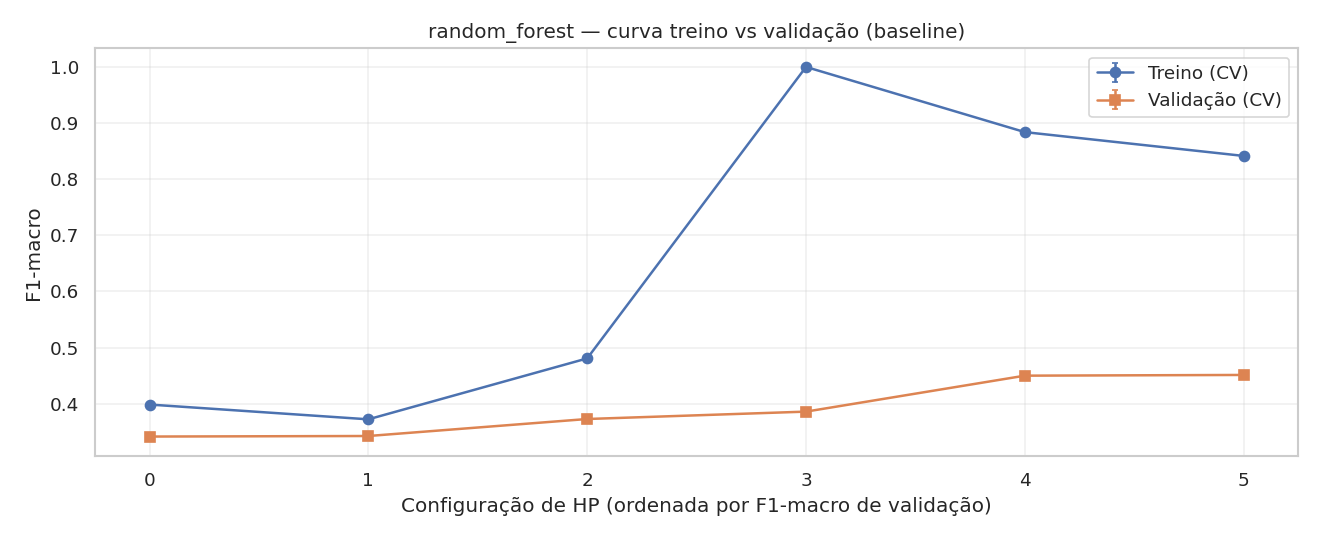
\includegraphics[width=\linewidth]{reports/figures/random_forest__baseline__train_vs_val.png}
  \caption{Random Forest (overfit).}
\end{subfigure}
\begin{subfigure}{0.49\linewidth}
  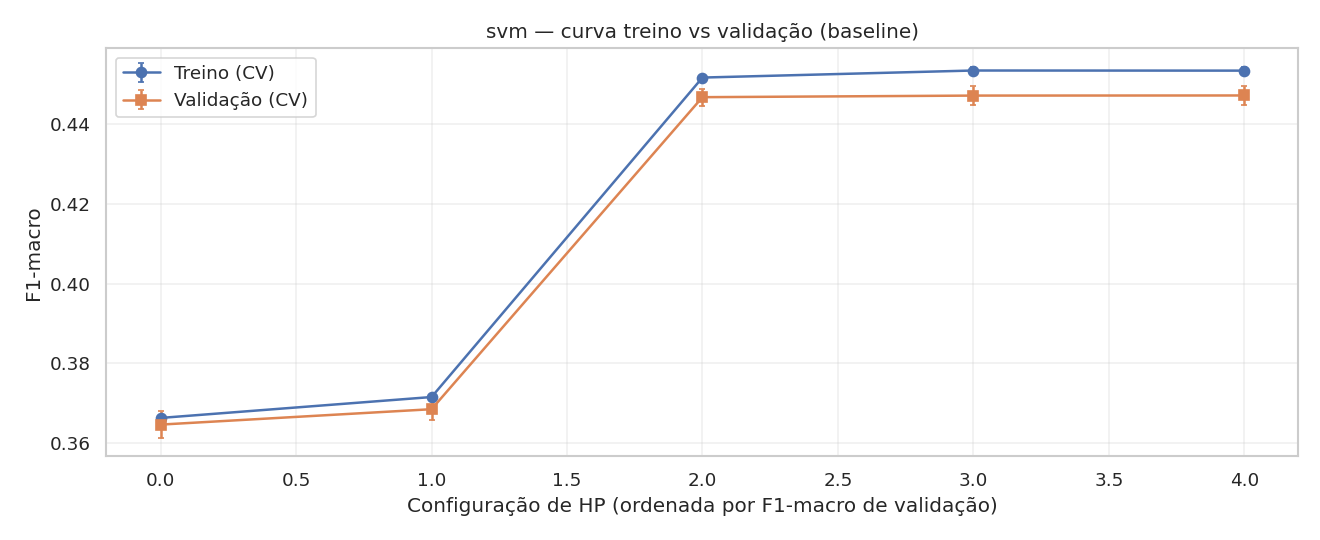
\includegraphics[width=\linewidth]{reports/figures/svm__baseline__train_vs_val.png}
  \caption{SVM (viés/underfit).}
\end{subfigure}
\caption{Curvas treino vs.\ validação (baseline). Os 50 gráficos completos estão em \texttt{reports/figures/}.}
\label{fig:curvas}
\end{figure}

\subsection{Comparação pareada baseline vs variantes}
Para cada par (modelo, variante) aplicamos Wilcoxon pareado \emph{e} paired t-test sobre os mesmos 5 folds. Com apenas 5 folds, o Wilcoxon atinge no mínimo $p=0{,}0625$, nunca cruza 0{,}05, então a decisão de promover usa o paired t-test ($p_t$), reportando ambos por transparência. Das 40 comparações, \textbf{17 promovem a variante} ($\Delta>0$ e $p_t<0{,}05$). A Tabela~\ref{tab:pair} resume os extremos.

O padrão é nítido e simétrico: \textbf{reamostragem (SMOTE/undersample) ajuda modelos sem balanceamento embutido}, LVQ ($+0{,}152$ com undersample!), Comitê de MLPs ($+0{,}041$ com SMOTE), MLP, e os boostings com undersample, mas \textbf{degrada os que já usam} \texttt{class\_weight="balanced"} (RF $-0{,}021$, SVM $-0{,}019$ com SMOTE). O Stacking+SMOTE é o pior caso ($-0{,}028$), coerente com a ressalva de que sua CV interna gera meta-features sobre dados sintéticos. RobustScaler é praticamente nulo (árvores/SVM já invariantes a escala) e TargetEncoder degrada modelos sensíveis a representação (K-NN, MLP).

\begin{table}[h]\centering
\small
\begin{tabular}{llrrr}
\toprule
\textbf{Modelo} & \textbf{Variante} & $F1_{\text{base}}$ & $F1_{\text{var}}$ & $\Delta$ ($p_t$) \\
\midrule
\multicolumn{5}{l}{\textit{Promovidas ($\Delta>0$, $p_t<0{,}05$)}}\\
LVQ            & undersample & 0{,}265 & 0{,}417 & $+$0{,}152 ($<$0{,}001) \\
LVQ            & SMOTE       & 0{,}265 & 0{,}392 & $+$0{,}127 ($<$0{,}001) \\
Comitê de MLPs & SMOTE      & 0{,}408 & 0{,}449 & $+$0{,}041 ($<$0{,}001) \\
MLP            & SMOTE       & 0{,}412 & 0{,}439 & $+$0{,}027 (0{,}005) \\
Stacking       & undersample & 0{,}417 & 0{,}438 & $+$0{,}022 ($<$0{,}001) \\
XGBoost        & undersample & 0{,}424 & 0{,}442 & $+$0{,}018 ($<$0{,}001) \\
LightGBM       & undersample & 0{,}420 & 0{,}437 & $+$0{,}017 (0{,}001) \\
\midrule
\multicolumn{5}{l}{\textit{Degradam ($\Delta<0$, $p_t<0{,}05$)}}\\
Stacking       & SMOTE       & 0{,}417 & 0{,}389 & $-$0{,}028 ($<$0{,}001) \\
Random Forest  & SMOTE       & 0{,}451 & 0{,}430 & $-$0{,}021 ($<$0{,}001) \\
SVM            & SMOTE       & 0{,}447 & 0{,}428 & $-$0{,}019 ($<$0{,}001) \\
Random Forest  & undersample & 0{,}451 & 0{,}433 & $-$0{,}018 ($<$0{,}001) \\
\bottomrule
\end{tabular}
\caption{Comparação pareada baseline vs.\ variante (Wilcoxon e paired t-test sobre 5 folds; $p_t$ = paired t-test). Tabela completa das 40 comparações em \texttt{reports/cv\_results/paired\_baseline\_vs\_variants.csv}.}
\label{tab:pair}
\end{table}

\begin{figure}[h]
  \centering
  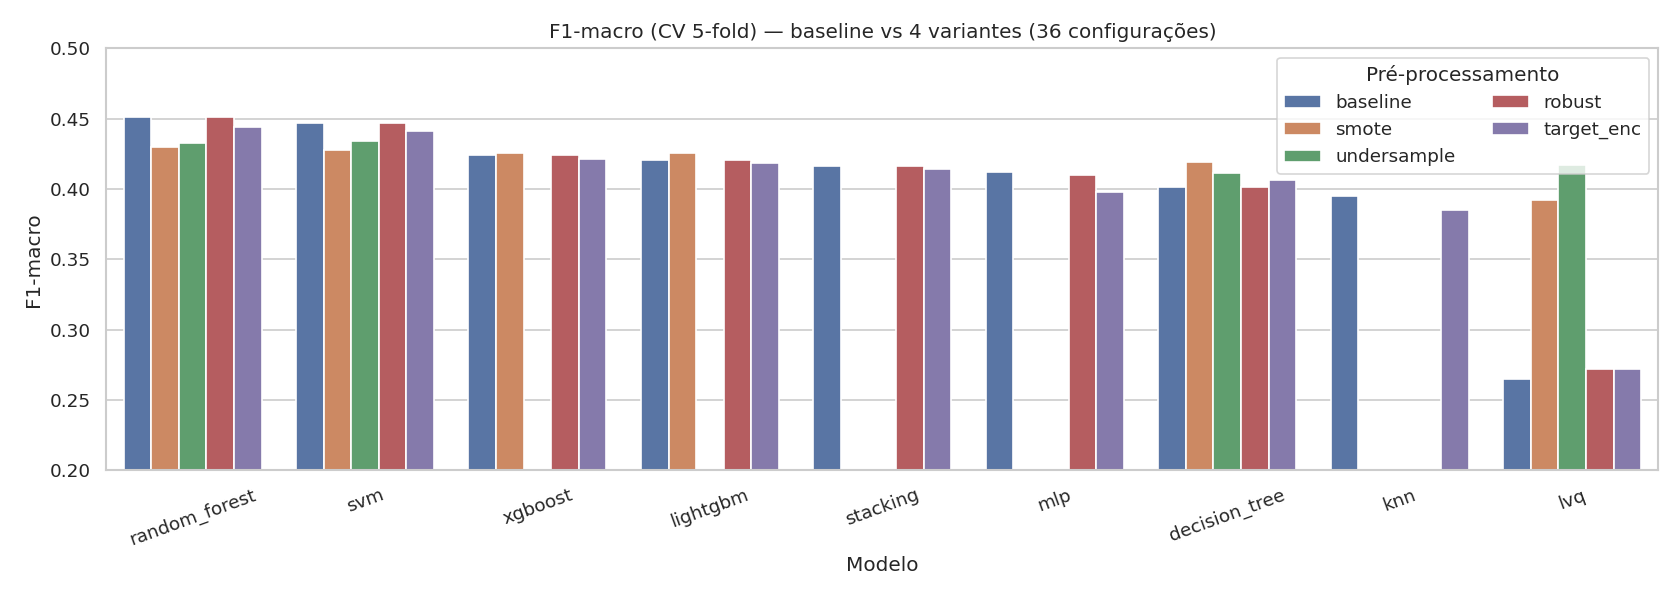
\includegraphics[width=0.95\linewidth]{reports/figures/baseline_vs_variants_f1.png}
  \caption{F1-macro (média dos 5 folds) por modelo e pré-processamento.}
  \label{fig:f1_bars}
\end{figure}

\subsection{Seleção do modelo final}
O ranking unificado das 50 combinações coloca o \textbf{Random Forest} no topo, com F1-macro de validação \textbf{0{,}4513 $\pm$ 0{,}0028}, empate técnico entre baseline e RobustScaler ($\Delta<10^{-3}$, sem significância). A busca selecionou \texttt{n\_estimators=200}, \texttt{max\_depth=20}, \texttt{max\_features="log2"}, \texttt{min\_samples\_leaf=1} e \texttt{class\_weight="balanced"}; este último ataca o desbalanceamento dentro do classificador, explicando por que reamostragem o \emph{piora}. O 2º lugar é o Comitê de MLPs+SMOTE (0{,}4490) e o 3º o SVM (0{,}4471), ambos sem diferença significativa para o RF. O desempate seguiu o briefing: o RF tem inferência em $\sim$ms/amostra, fornece importância de variáveis para auditoria de viés e é robusto a escala, escolhemos a variante \texttt{RobustScaler} (equivalente em F1 e mais estável às caudas longas das contagens). O gap treino$-$validação alto (0{,}84 vs 0{,}45) revela capacidade ociosa, mas a variância mínima entre folds ($\sigma=0{,}003$) confirma estabilidade.

\subsection{Matrizes de confusão por algoritmo}
Para cada algoritmo geramos a matriz de confusão normalizada do melhor modelo no baseline \emph{e} na sua melhor variante, a partir de predições \emph{out-of-fold} (\texttt{cross\_val\_predict}, mesma CV das buscas), portanto métricas de treino/validação, sem tocar o teste. As 20 figuras estão em \texttt{reports/figures/cm\_\_<modelo>\_\_<tag>.png}; a Figura~\ref{fig:cm_rf} mostra o vencedor. Em todos os modelos o padrão se repete: a classe minoritária \texttt{<30} é a mais confundida (majoritariamente classificada como \texttt{>30} ou \texttt{NO}), o que motiva a calibração de limiar no deployment.

\begin{figure}[h]
\centering
\begin{subfigure}{0.49\linewidth}
  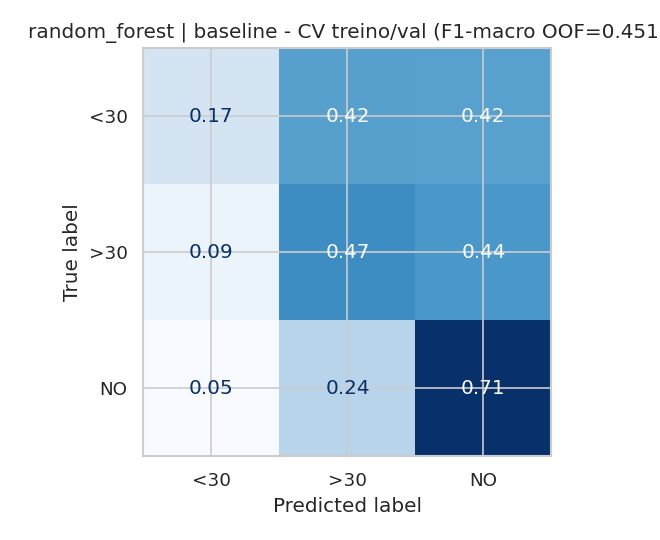
\includegraphics[width=\linewidth]{reports/figures/cm__random_forest__baseline.png}
  \caption{RF baseline.}
\end{subfigure}
\begin{subfigure}{0.49\linewidth}
  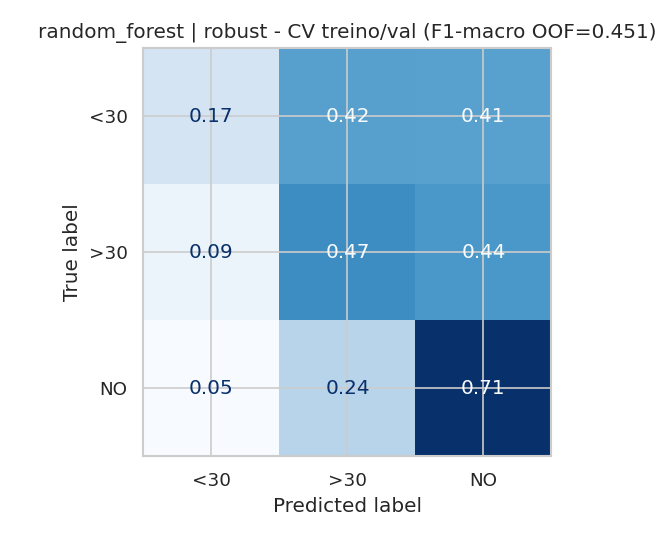
\includegraphics[width=\linewidth]{reports/figures/cm__random_forest__robust.png}
  \caption{RF RobustScaler (variante vencedora).}
\end{subfigure}
\caption{Matrizes de confusão normalizadas do Random Forest (out-of-fold, treino/validação).}
\label{fig:cm_rf}
\end{figure}

\subsection{Por que F1-macro $\sim$0,45 é competitivo}
O F1-macro $\sim$0,45 não reflete deficiência de modelagem, e sim o teto de informação do problema. A fronteira \texttt{<30} vs.\ \texttt{>30} é clinicamente arbitrária (readmitir em 28 ou 32 dias é praticamente indistinguível), o alvo depende fortemente de fatores ausentes do dataset (suporte social, adesão, acesso pós-alta), e o F1-\emph{macro} pondera igualmente a classe minoritária \texttt{<30}, a mais difícil. O ROC-AUC macro de 0{,}674 quantifica esse sinal fraco porém real, em linha com a literatura: estudos de readmissão em 30 dias sobre este mesmo dataset reportam tipicamente AUC entre 0{,}65 e 0{,}70.

Resultados aparentemente superiores na literatura quase sempre decorrem de (i) \emph{binarização} do alvo (\texttt{<30} vs.\ resto), tarefa mais fácil e não comparável; (ii) reporte de \emph{acurácia}, dominada pela classe majoritária \texttt{NO} (54\%), em vez de F1-macro; ou (iii) \emph{vazamento} (reamostragem/codificação antes do split, ou uso do teste na seleção). Valores honestos de F1-macro trinário acima de $\sim$0{,}55 nesse dataset são suspeitos de uma dessas causas.

Quanto a \emph{deep learning}: para dados tabulares predominantemente categóricos como este, modelos baseados em árvore seguem superando redes profundas\footnote{Grinsztajn, Oyallon \& Varoquaux. \emph{Why do tree-based models still outperform deep learning on tabular data?} NeurIPS 2022. \url{https://arxiv.org/abs/2207.08815}}. O próprio estudo confirma isso internamente --- MLP (0{,}412), Comitê de MLPs (0{,}408) e Stacking (0{,}417) ficaram \emph{abaixo} do Random Forest (0{,}451). O ganho real viria de engenharia de características com domínio (índices de comorbidade dos códigos ICD, padrões de troca de medicação, recência de visitas), aprendizado sensível a custo, reformulação binária com calibração de limiar para o objetivo operacional, ou dados externos --- não de uma arquitetura mais complexa. A contribuição do trabalho está, portanto, no \textbf{rigor metodológico} (split intocado, 50 combinações comparadas com teste pareado, sem vazamento), que separa este resultado dos números inflados frequentes na literatura aplicada.

\section{Avaliação no conjunto de teste}
Refit do Random Forest (RobustScaler, \texttt{class\_weight="balanced"}) em todo o treino e \emph{única} predição no teste isolado (destravado pelo token na Seção 9 do notebook):
\begin{itemize}
  \item \textbf{F1-macro (teste) = 0{,}4553}; F1-macro (CV) = 0{,}4513 $\pm$ 0{,}0028; \textbf{$\Delta$ = $+$0{,}0041}.
  \item Balanced accuracy = 0{,}4530; ROC-AUC macro = 0{,}6737; PR-AUC macro = 0{,}4739.
\end{itemize}

\begin{table}[h]\centering
\small
\begin{tabular}{lcccc}
\toprule
\textbf{Classe} & \textbf{Precisão} & \textbf{Recall} & \textbf{F1} & \textbf{Suporte} \\
\midrule
\texttt{<30}    & 0{,}241 & 0{,}196 & 0{,}216 & 2.272 \\
\texttt{>30}    & 0{,}477 & 0{,}479 & 0{,}478 & 7.109 \\
\texttt{NO}     & 0{,}661 & 0{,}684 & 0{,}672 & 10.973 \\
\midrule
\textbf{macro}  & 0{,}459 & 0{,}453 & 0{,}455 & 20.354 \\
\bottomrule
\end{tabular}
\caption{Relatório de classificação no teste (Random Forest, RobustScaler).}
\label{tab:test}
\end{table}

\begin{figure}[h]
\centering
\begin{subfigure}{0.32\linewidth}
  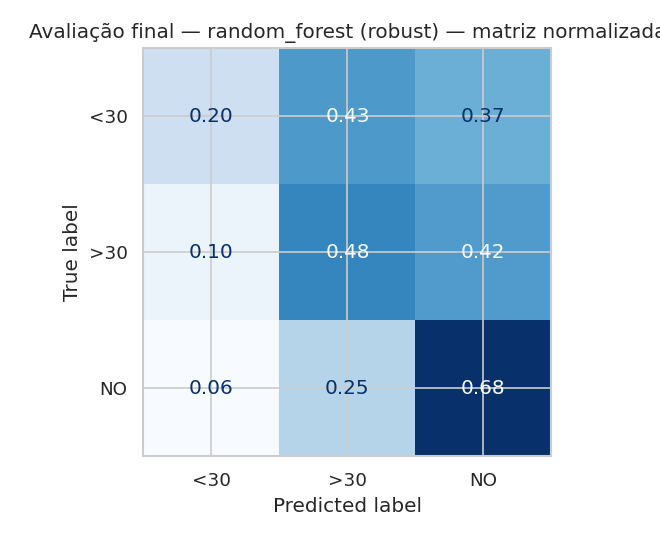
\includegraphics[width=\linewidth]{reports/figures/final_confusion.png}
  \caption{Matriz normalizada.}
\end{subfigure}
\begin{subfigure}{0.32\linewidth}
  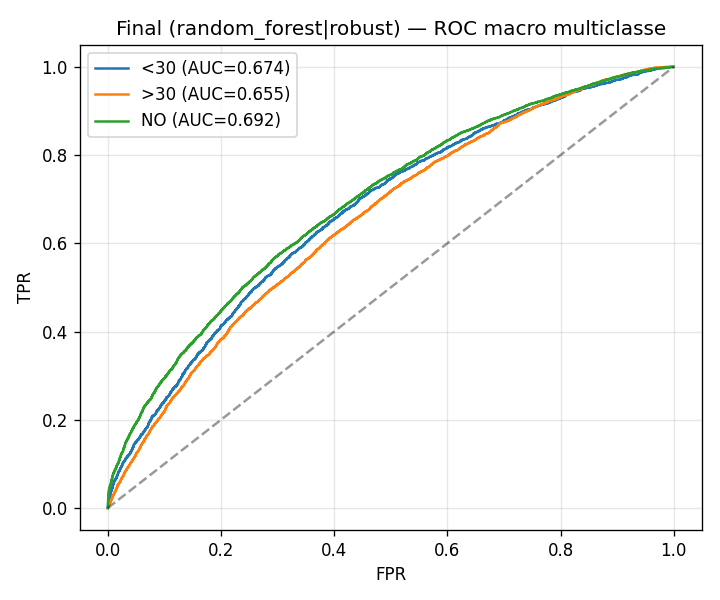
\includegraphics[width=\linewidth]{reports/figures/final__roc.png}
  \caption{ROC macro.}
\end{subfigure}
\begin{subfigure}{0.32\linewidth}
  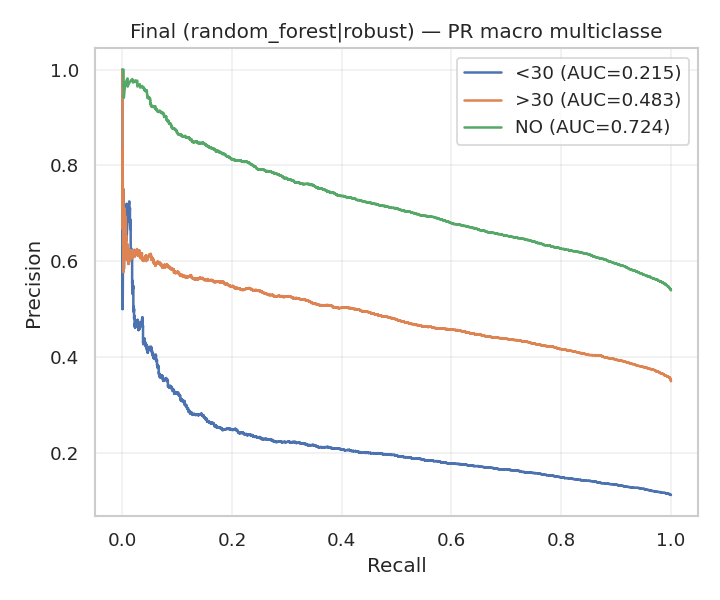
\includegraphics[width=\linewidth]{reports/figures/final__pr.png}
  \caption{PR macro.}
\end{subfigure}
\caption{Avaliação final no teste, Random Forest (RobustScaler).}
\label{fig:final}
\end{figure}

\textbf{Gap CV$\rightarrow$teste e leitura por classe.} O $\Delta$ de apenas $+0{,}004$ entre validação e teste confirma que a seleção via CV \emph{não} sofreu overfit ao processo de busca, o pipeline generaliza. A classe \texttt{NO} domina o acerto (F1=0{,}672); a crítica \texttt{<30} tem F1=0{,}216 e \textbf{recall de só 0{,}196}, ou seja, $\approx$80\% dos pacientes de alto risco passam despercebidos no ponto de operação padrão. Isso reforça que, em produção, o limiar sobre \texttt{predict\_proba(<30)} deve ser calibrado para elevar esse recall até o teto da fila de acompanhamento, aceitando mais falsos positivos (custo operacional menor que o de uma readmissão precoce não assistida).

\section{Deployment, riscos e monitoramento}

\subsection{Cenário de uso e integração}
O modelo é entregue como um serviço de escore acionado na alta de cada paciente diabético, integrado ao prontuário eletrônico. A predição alimenta uma fila de acompanhamento ativo: pacientes sinalizados como \texttt{<30} recebem ligação de enfermagem em 48h, agendamento de retorno em 7 dias e revisão da farmacoterapia. O escore é apoio à decisão clínica, nunca substituição: a equipe pós-alta pode incluir ou remover pacientes da fila por julgamento clínico, e toda decisão automatizada fica registrada para auditoria. A inferência do Random Forest custa da ordem de milissegundos por paciente, compatível com a restrição operacional de latência do briefing ($<200$ ms).

\subsection{Ponto de operação e calibração de limiar}
A seleção do modelo otimizou F1-macro, mas a operação exige um ajuste adicional. No limiar padrão (\texttt{argmax} da probabilidade), o recall da classe \texttt{<30} é de apenas 0{,}196, ou seja, cerca de 80\% dos pacientes de alto risco não são sinalizados, o que é inaceitável dado o custo assimétrico do falso negativo. Por isso o ponto de operação é definido por calibração de limiar sobre \texttt{predict\_proba(<30)}: baixamos o limiar para elevar o recall da classe crítica até o teto de capacidade da fila ($\approx$30 pacientes/dia na hipótese de uso), aceitando mais falsos positivos. O custo de um falso positivo (uma ligação de acompanhamento desnecessária) é muito menor que o de um falso negativo (readmissão precoce sem suporte), então a curva precisão/recall, e não o F1-macro, guia o limiar final. Esse limiar é revisto periodicamente conforme a capacidade do time muda.

\subsection{Riscos e mitigações}
\begin{itemize}
  \item \textbf{Viés demográfico.} As variáveis \texttt{race} (com nível ``Other'' e alta ausência), \texttt{gender} e \texttt{age} podem carregar viés histórico de acesso e tratamento. Mitigação: auditoria de \emph{disparate impact ratio} por subgrupo antes do go-live e relatório mensal de F1-macro e recall(\texttt{<30}) estratificados por raça, gênero e faixa etária; bloqueio de promoção se houver disparidade material entre subgrupos.
  \item \textbf{Falso negativo da classe \texttt{<30}.} É o erro de maior custo clínico. Mitigação: limiar conservador (item anterior), além de revisão clínica por exceção dos casos de borda (probabilidade próxima ao limiar) encaminhados ao time.
  \item \textbf{Drift de população.} Expansão para nova unidade ou mudança no perfil de pacientes pode invalidar o pipeline. Mitigação: monitoramento semanal de drift (PSI/KS) nas variáveis de maior peso (\texttt{number\_inpatient}, \texttt{discharge\_disposition\_id}, \texttt{diag\_*} agrupado, número de medicações).
  \item \textbf{Privacidade.} Dados clínicos sensíveis. Mitigação: treino offline sobre dados pseudonimizados, inferência restrita ao escopo da própria conta hospitalar, retenção mínima e sem persistência de dados crus fora de \texttt{data/raw/}.
  \item \textbf{Qualidade e dependência de dados.} O pipeline assume a codificação ICD-9 e os identificadores operacionais do dataset original; mudanças de padrão (por exemplo, migração para ICD-10) quebram o pré-processamento. Mitigação: validação de schema na entrada e fallback para imputação quando uma categoria nova aparece (\texttt{handle\_unknown="ignore"} no OneHotEncoder).
\end{itemize}

\subsection{Plano de monitoramento}
\begin{itemize}
  \item \textbf{Desempenho:} F1-macro e recall(\texttt{<30}) mensais sobre os pacientes com follow-up completo (rótulo disponível 30+ dias após a alta), estratificados por unidade e faixa etária.
  \item \textbf{Drift de dados:} PSI semanal nas 15 variáveis de maior importância; PSI $>0{,}2$ em qualquer uma dispara revisão.
  \item \textbf{Métricas de produto:} taxa de aceitação do alerta pela equipe clínica, taxa de comparecimento à consulta agendada motivada pelo alerta, e latência de inferência.
\end{itemize}

\subsection{Retreinamento e governança}
O retreinamento é disparado quando: (a) o PSI ultrapassa $0{,}25$ em $\geq$3 das variáveis de maior peso, (b) o F1-macro mensal de produção cai mais de $0{,}05$ em relação ao F1-macro do teste reportado, ou (c) trimestralmente, como rotina. O pipeline de retreinamento reusa o \texttt{main.ipynb} (invalidando o cache do modelo vencedor), e o novo modelo entra em produção via \emph{canary release} de 10\% por duas semanas, com comparação A/B contra a versão vigente antes da promoção total. Cada versão de modelo é versionada junto com seu \texttt{cv\_results\_}, hiperparâmetros e métricas de teste, garantindo rastreabilidade e \emph{rollback}.

\subsection{Limitações}
O recall padrão da classe \texttt{<30} é baixo (0{,}196), o que torna a calibração de limiar indispensável, não opcional. A fronteira clínica de 30 dias é arbitrária, limitando o teto de desempenho independentemente do modelo (ver a discussão na Seção~5). Por fim, o modelo foi treinado em dados de 1999 a 2008 de hospitais americanos; sua transferência para outra população ou época exige revalidação antes do uso.

\section{Reprodutibilidade e ferramentas}
\subsection{Ferramentas}
\begin{itemize}
  \item Python 3.12, gerenciado por \texttt{uv} (\texttt{uv.lock} versionado).
  \item Pipelines em \texttt{scikit-learn} 1.8 (com \texttt{imbalanced-learn} 0.14 para SMOTE).
  \item XGBoost 3.2 (GPU/CUDA quando disponível), LightGBM 4.6, sklvq 0.1.2 (com shim \texttt{PatchedGLVQ}).
\end{itemize}

\subsection{Reprodução}
\begin{verbatim}
uv sync
uv run jupyter nbconvert --to notebook --execute main.ipynb \
                          --output main.executed.ipynb
\end{verbatim}
A primeira execução popula \texttt{reports/cv\_results/} (CSVs por modelo $\times$ variante) e \texttt{reports/figures/} (curvas, matriz, ROC/PR). Execuções subsequentes reusam o cache (\texttt{get\_or\_run\_search}).

\subsection{Uso de IA generativa}
Em conformidade com a Seção 14 das exigências, declaramos o uso do assistente de programação Claude (Anthropic, Opus 4.7 e 4.8) durante o desenvolvimento, para apoio em codificação, revisão e documentação. Decisões metodológicas (split estratificado, escolha de métrica, escolha de algoritmos e variantes, leitura crítica dos resultados, e revisão final deste relatório) foram conduzidas pela equipe.

\end{document}
